Da die Minispiele alle einem ähnlichen Grundaufbau folgen, bietet es sich an, diesen objektorientiert und modular zu implementieren, um Redundanz zu vermeiden.
Dieser Grundaufbau besteht aus den folgenden Klassen:

\begin{itemize}
    \item \texttt{LevelScene}
    \item \texttt{LevelSelectorScene}
    \item \texttt{MinigameEndScene}
    \item \texttt{Minigames}
\end{itemize}

\paragraph{LevelScene} Diese abstrakte Klasse ist eine Erweiterung der \texttt{BaseScene} und stellt allgemeine Variablen und Methoden zur Verfügung.
Sie beinhaltet:

\begin{sloppypar}
    \begin{itemize}
        \item \texttt{REWARD}: Ein \texttt{ItemObject}, welches die Spielenden nach erfolgreichendem Beenden des Levels erhalten.
            Es wird mit Hilfe der Methode \texttt{getMinigameReward} der \texttt{ItemObject}-Klasse generiert.
        \item Ein \texttt{BackdropObject} welches das zur Fachschaft gehörende Hintergrundbild beinhaltet.
        \item \texttt{exitButton}: Ein \texttt{ButtonObject}, welches das Verlassen des Minispiels mittels Entfernen der obersten zwei Scenen des \texttt{SceneStack}, hier \texttt{LevelScene} und \texttt{LevelSelectorScene}, ermöglicht.
        \item \texttt{menuButton}: Ein \texttt{ButtonObject}, welches die Rückkehr zur Level-Auswahl mittels Entfernen der obersten Scene des \texttt{SceneStack}, in diesem Fall die entsprechende \texttt{LevelScene}, ermöglicht.
        \item \texttt{reset()}: Eine abstrakte Methode, welche das Zurücksetzten eines Levels ermöglichen soll.
            Dafür wird sie von den Leveln der Fachschaften implementiert, welche dann je nach Minispiel eine komplett neue Instanz von sich erstellen, oder nur einzelne Elemente neu generieren bzw. zurücksetzen.
        \item \texttt{levelWon()}: Eine Prozedur, welche eine Instanz der \texttt{MinigameEndScene} auf den Szenenstapel hinzufügt und \texttt{REWARD} in das Inventar der Spielfigur übergibt.
        \item \texttt{levelLost()}: Eine Prozedur, durch deren Aufruf eine Instanz der \texttt{MinigameEndScene} auf den \texttt{SceneStack} gepushed wird.
        \item \texttt{LevelScene(Department department, int level)}: Der Konstruktor der Klasse, welcher mit Hilfe seiner Parameter das Hintergrundbild lädt und die Knöpfe platziert.
    \end{itemize}
\end{sloppypar}

\paragraph{LevelSelectorScene} Diese Klasse ist eine Erweiterung der \texttt{BaseScene} und verknüpft, neben anderen Methoden, jeweils drei \texttt{LevelScene}s miteinander.
Sie beinhaltet:

\begin{sloppypar}
    \begin{itemize}
        \item \texttt{LEVELS}: Ein \texttt{LevelScene}-Array, welches die drei Level beinhaltet.
        \item Ein \texttt{BackdropObject} welches das Hintergrundbild beinhaltet.
        \item \texttt{exitButton}: Ein \texttt{ButtonObject}, welches das Verlassen des Minispiels mittels Entfernen der obersten Scene des \texttt{SceneStack} (\texttt{LevelSelectorScene}) ermöglicht.
        \item \texttt{buttonLevel1}: Ein \texttt{ButtonObject}, welches die erste in \texttt{LEVELS} gespeicherte \texttt{LevelScene} auf den \texttt{SceneStack} pushed.
        \item \texttt{buttonLevel2}: Ein \texttt{ButtonObject}, welches die zweite in \texttt{LEVELS} gespeicherte \texttt{LevelScene} auf den \texttt{SceneStack} pushed.
        \item \texttt{buttonLevel3}: Ein \texttt{ButtonObject}, welches die dritte in \texttt{LEVELS} gespeicherte \texttt{LevelScene} auf den \texttt{SceneStack} pushed.
        \item \texttt{LevelSelectorScene(LevelScene level1, LevelScene level2, LevelScene level3)}: Der Konstruktor der Klasse, welcher mit Hilfe seiner Parameter das Hintergrundbild lädt und die Knöpfe platziert.
    \end{itemize}
\end{sloppypar}

\paragraph{MinigameEndScene} Diese Klasse ist eine Erweiterung der \texttt{BaseScene} und ist für das Ende eines Levels zuständig.
Sie beinhaltet:

\begin{sloppypar}
    \begin{itemize}
        \item Ein \texttt{BackdropObject} welches einen schwarzen, semi-transparenten Hintergrund beinhaltet, um das Level zu verdunkeln.
        \item \texttt{banner}: Ein \texttt{BaseObject}, welches entweder den Schriftzug \glqq GEWONNEN\grqq{} oder \glqq VERLOREN\grqq{} darstellt.
        \item \texttt{rewardContainer}: Ein \texttt{BaseObject}, welches als Rahmen für das gewonnene Item dient.
            Es wird nur gezeichnet, falls das Level gewonnen wurde.
        \item \texttt{rewardItem}: Ein \texttt{BaseObject}, welches das gewonnene Item darstellt.
            Es wird nur gezeichnet, falls das Level gewonnen wurde.
        \item \texttt{exitButton}: Ein \texttt{ButtonObject}, welches das Level mittels der Prozedur \texttt{resetMinigameLevel} der \texttt{Minigames}-Klasse, auf die später noch einmal eingengangen wird, ohne es direkt neu zu starten zurücksetzt und das Minispiel mittels Entfernen der obersten Scene des \texttt{SceneStack} (nach Zurücksetzen: \texttt{LevelSelectorScene}) verlässt.
        \item \texttt{menuButton}: Ein \texttt{ButtonObject}, welches das Level mittels der Prozedur \texttt{resetMinigameLevel} der \texttt{Minigames}-Klasse ohne es direkt neu zu starten zurücksetzt.
        \item \texttt{retryButton}: Ein \texttt{ButtonObject}, welches das Level mittels der Prozedur \texttt{resetMinigameLevel} der \texttt{Minigames}-Klasse zurücksetzt.
        \item \texttt{MinigameEndScene(boolean won, int level, ItemObject reward)}: Der Konstruktor der Klasse, welcher mit Hilfe seiner Parameter das Hintergrundbild, das Banner und gegebenenfalls die Belohnung lädt, sowie die Knöpfe platziert.
    \end{itemize}
\end{sloppypar}

\paragraph{Minigames} Diese Klasse ist statisch und stellt Methoden zum Starten und Zurücksetzen der Minispiele zur Verfügung.
Sie beinhaltet:

\begin{sloppypar}
    \begin{itemize}
        \item \texttt{generateMinigame(Department department)}: Eine Methode, welche abhängig von der als Parameter gegebenen Fachschaft eine \texttt{LevelSelectorScene} mit den passenden Leveln zurückgibt.
        \item \texttt{resetMinigameLevel(int level, boolean autoRetry)}: Eine Prozedur, welche die obersten zwei Szenen des \texttt{SceneStack} - \texttt{MinigameEndScene} und \texttt{LevelScene}, da diese Methode nur nach dem Beenden eines Minispieles aufgerufen wird - entfernt und das als Parameter gegebene Level der jetzt oben liegenden \texttt{LevelSelectorScene} mittels der \texttt{reset}-Methode des Levels zurücksetzt.
            Falls der Parameter \texttt{autoRetry} wahr ist, wird zusätzlich das zurückgesetzte Level auf den \texttt{SceneStack} gepushed.
        \item \texttt{Minigames}: Der Konstruktor der Klasse, welcher leer ist und als \texttt{private} deklariet ist, da er nicht aufgerufen werden soll.
    \end{itemize}
\end{sloppypar}

Um also ein Minispiel für eine Fachschaft zu implementieren, müssen folgende Dinge geschehen:

\begin{sloppypar}
    \begin{enumerate}
        \item Erweiterung der \texttt{LevelScene}, um die Funktionsweise des Spieles zu implementieren.
        \item Hinzufügen von weiteren Klassen oder Resourcen, die von der erweiterten \texttt{LevelScene} benötigt werden.
        \item Hinzufügen eines \texttt{ButtonObject} in der den Raum der Fachschaft repräsentierenden Szene (beispielsweise \texttt{MatheraumScene}), welches die von \texttt{Mingames.generateMinigame} erstellte \texttt{LevelSelectorScene} auf den \texttt{SceneStack} pushed.
    \end{enumerate}
\end{sloppypar}

In den folgenden Abschnitten sind diese fachschaftspezifischen Erweiterungen erklärt.

\subsubsection{Informatik}

\begin{sloppypar}
    Für das Minispiel der Fachschaft Informatik wurde die \texttt{LevelScene} zur \texttt{ComputerScienceLevelScene} erweitert, um das Zeichnen, Auswählen und Überprüfen der Logikgatter, sowie das Zeichnen des Schaltkreises zu ermöglichen.
    Außerdem wurde ein \texttt{LogicGate}-Enum, welches die Gatter verwaltet, sowie ein \texttt{ComputerSciencePuzzle}-Enum, das die Schaltkreise bereit stellt, hinzugefügt.    
\end{sloppypar}

\paragraph{LogicGate} Die Implementierung mittels einer Enumeration bietet sich an, da vorgegebene Logikgatter definiert werden, die nicht verändert oder durch weitere ergänzt werden sollen.
Jede Enum-Konstante speichert zusätzlich noch ein Bild, welches das Gatter repräsentiert.
Zusätzlich werden noch Methoden zur Generierung einer zufälligen Auswahl an Logikgattern, welche als Antwortmöglichkeiten fungieren, implementiert.
Die Klasse beinhaltet:

\begin{sloppypar}
    \begin{itemize}
        \item \texttt{SPRITE}: Ein \texttt{java.awt.Image}, das das zum Logikgatter gehörende Bild speichert.
        \item \texttt{getRandom()}: Eine statische Methode, welche eine zufällige Enum-Konstante mittels der \texttt{java.util.Random}-Klasse zurückgibt.
        \item \texttt{getRandomArray(int length, LogicGate[] includedGates)}: Eine statische Methode, welche ein zufällig generiertes Array an Enum-Konstanten der Länge \texttt{length} zurückgibt, welches jedes Gatter höchstens einmal und alle in \texttt{includedGates} gegebenen Gatter enthält. 
        \item \texttt{LogicGate(String path)}: Der Konstruktor der Klasse, welcher nur von der Klasse selbst bei der Initialisierung der Konstanten aufgerufen wird.
            Er speichert das durch \texttt{path} gegebene Bild in \texttt{SPRITE}.
    \end{itemize}
\end{sloppypar}

Die \texttt{getRandomArray}-Methode ist zur näheren Erklärung im Folgenden dargestellt.

\begin{lstlisting}[caption=getRandomArray-Methode, label=lst:mggetRandomArray, captionpos=t, language=Java]
public static LogicGate[] getRandomArray(
    int length, LogicGate[] includedGates
) {
    // Das zu generierende Array
    LogicGate[] out = new LogicGate[length];
    // Indizes der Gatter, die beinhaltet werden sollen
    List<Integer> includedGatesIdx = new ArrayList<>();

    // Abbruch, falls mehr Gatter zurückgegeben werden sollen,
    // als Enum-Konstanten existieren.
    if (length > LogicGate.values().length) return null;

    // Abbruch, falls die Länge der zu beinhaltenden Gatter
    // größer ist, als die der gesamten Liste.
    if (includedGates.length > length) return null;

    // Generierung der Indizes der Gatter, die beinhaltet
    // werden sollen
    for (int i = 0; i < includedGates.length; i++) {
        // zufälliger Index
        int r = new Random().nextInt(length);

        // Neuer zufälliger Index, solange der alte bereits
        // generiert wurde
        while (includedGatesIdx.contains(r)) {
            r = new Random().nextInt(length);
        }

        // Hinzufügen des Indexes
        includedGatesIdx.add(r);
    }

    // Generierung des Logikgatter-Arrays
    for (int i = 0; i < length; i++) {
        // Überprüfung, ob an Index i ein gegebenes Gatter
        // platziert oder ein neues Gatter generiert werden soll
        if (includedGatesIdx.contains(i)) {
            // Hinzufügen des gegebenen Gatters an dem
            // in includedGatesIdx gespeicherten Index
            out[i] = includedGates[includedGatesIdx.indexOf(i)];
        } else {
            // Zufälliges Gatter
            LogicGate rGate = getRandom();
            // Neues zufälliges Gatter, solange das alte
            // entweder in den gegebenen Gattern oder
            // in dem bereits generierten Array enthalten ist.
            while (
                Arrays.asList(includedGates).contains(rGate) ||
                Arrays.asList(out).contains(rGate)
            ) {
                rGate = getRandom();
            }

            // Hinzufügen des Gatters
            out[i] = rGate;
        }
    }

    // Rückgabe des fertigen Arrays
    return out;
}
\end{lstlisting}

\paragraph{ComputerSciencePuzzle} Die Implementierung mittels einer Enumeration bietet sich an, da vorgegebene Schaltkreise definiert werden, die nicht verändert oder durch weitere ergänzt werden können.
Sie beinhaltet:

\begin{sloppypar}
    \begin{itemize}
        \item \texttt{PUZZLES}: Ein statisches, zweidimensionales \texttt{ComputerSciencePuzzle}-Array, welches für jedes Level die zugehörigen Enum-Konstanten speichert.
        \item \texttt{SPRITE}: Ein \texttt{java.awt.Image}, das das zum Puzzle gehörende Bild speichert.
        \item \texttt{SOLUTION}: Ein \texttt{LogicGate}-Array, das die im Schaltkreis abgedeckten Logikgatter enthält.
        \item \texttt{ANSWERS}: Ein \texttt{LogicGate}-Array, das die zur Auswahl stehenden Antwortmöglichkeiten beinhaltet.
        \item \texttt{getPuzzle(int level)}: Eine Methode, welche eine zufällige Enum-Konstante basierend auf dem gegebenen level, mittels der \texttt{java.util.Random}-Klasse zurückgibt.
        \item \texttt{ComputerSciencePuzzle(String path, LogicGate[] solution, int amountOfAnswers)}: Der Konstruktor der Klasse, welcher nur von der Klasse selbst bei der Initialisierung der Konstanten aufgerufen wird.
            Er speichert das durch \texttt{path} gegebene Bild in \texttt{SPRITE}, die Lösung \texttt{solution} in \texttt{SOLUTION} und generiert \texttt{ANSWERS} mittels \texttt{LogicGate.getRandomArray}.
    \end{itemize}
\end{sloppypar}

\paragraph{ComputerScienceLevelScene} Eine erweiterung der \texttt{LevelScene}, welche die grundlegenden Methoden des Informatik-Minispieles implementiert.
Sie beinhaltet:

\begin{sloppypar}
    \begin{itemize}
        \item \texttt{LEVEL}: Die ID des Levels.
        \item \texttt{PUZZLE}: Das \texttt{ComputerSciencePuzzle} des Levels.
        \item \texttt{ANSWER\_FRAMES}: Ein \texttt{BaseObject}-Array, das die Rahmen enthält, die um ausgewählte Antworten gezeichnet werden.
        \item \texttt{ACTIVE\_ANSWERS}: Ein \texttt{LogicGate}-Array, das die geantworteten Logikgatter enthält.
        \item \texttt{setAnswer(LogicGate gate, int x, int y)}: Eine Prozedur, welche für das Antworten verantwortlich ist.
            Sie setzt die Rahmen, aktualisiert die geantworteten Gatter, überprüft ob eine Lösung richtig oder falsch ist und beendet das Minispiel entsprechend.
        \item \texttt{reset()}: Die Implementierung der \texttt{LevelScene.reset}-Methode der. Sie gibt eine neu generierte \texttt{ComputerScienceLevelScene} zurück.
        \item \texttt{ComputerScienceLevelScene(int level)}: Der Konstruktor der Klasse, welcher alle Variablen initialisiet und die Gatter, sowie den Schaltkreis platziert.
    \end{itemize}
\end{sloppypar}

Die \texttt{setAnswer}-Methode ist zur näheren Erklärung im Folgenden als Struktogramm dargestellt.

\begin{figure}[H]
	\centering
	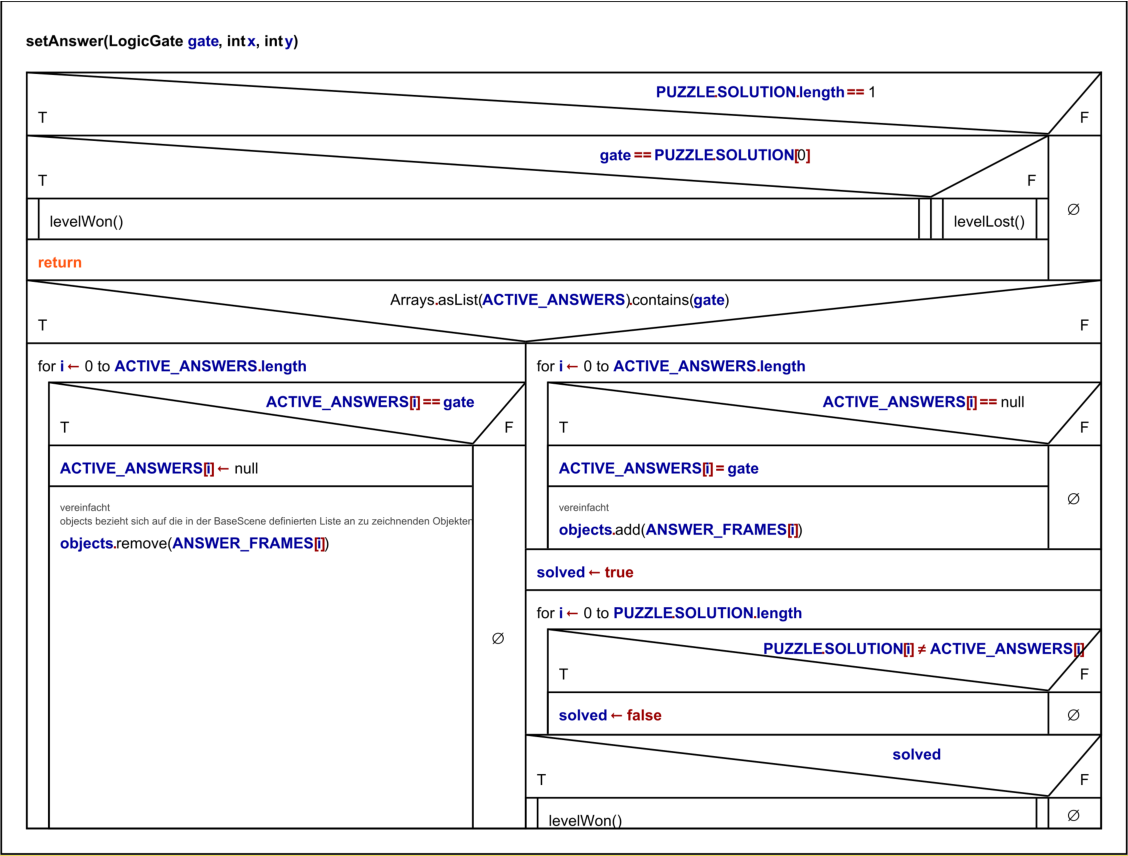
\includegraphics[width=1\textwidth]{bilder/StruktogrammSetAnswer.pdf}
	\caption{Struktogramm der setAnswer-Methode}
	\label{fig:mgsetAnswer}
\end{figure}

\subsubsection{Mathematik}

\begin{sloppypar}
    Für das Minispiel der Fachschaft Mathematik wurde die \texttt{LevelScene} zur \texttt{MathematicsLevelScene} erweitert, um das Zeichnen und Überprüfen der Tangramsteine, sowie das Zeichnen der Silhouette zu ermöglichen.
    Außerdem wurde eine \texttt{TangramPieceObject}-Klasse, welche die Tangramsteine verwaltet, sowie ein \texttt{MathematicsPuzzle}-Enum, das die Silhouette bereitstellt, hinzugefügt.    
\end{sloppypar}

\paragraph{TangramPieceObject} Diese Klasse erweitert das \texttt{BaseObject}.
Dadurch sorgt sie dafür, dass jeder Stein ein Bild besitzt und verschoben, sowie rotiert werden kann.
Sie beinhaltet:

\begin{sloppypar}
    \begin{itemize}
        \item \texttt{SPRITE\_PATH}: Der Pfad zum Bild des Steines.
        \item \texttt{originalWidth, originalHeight}: Die Ausgangsgröße des Steines.
        \item \texttt{rotation}: Die Rotation des Steines.
        \item \texttt{levelScene}: Die \texttt{MathematicsLevelScene}, zu der der Stein gehört.
        \item \texttt{isDragged}: Ein \texttt{boolean}, welcher speichert, ob der Stein gerade gezogen wird.
        \item \texttt{generatePieces()}: Eine statische Methode, die ein Array, welches alle Tangramsteine beinhaltet, zurückgibt.
        \item \texttt{setLevelScene(TangramPieceObject[] pieces, MathematicsLevelScene levelScene)}: Eine statische Prozedur, die bei jedem in \texttt{pieces} gegebenen Tangram-Stein die \texttt{levelScene} festlegt.
        \item \texttt{rotate(double degree)}: Eine Prozedur, die den Stein um den gegebenen Winkel in mathematisch negative Richtung dreht.
        \item \texttt{setRotation(double degree)}: Eine Prozedur, die den Stein so dreht, dass dieser eine Rotation von \texttt{degree} besitzt.
        \item \texttt{update(BaseScene scene)}: Eine Implementierung der \texttt{update}-Prozedur der \texttt{BaseScene}.
            Sie ermöglicht Verschiebung und Drehung des Tangram-Steines.
        \item \texttt{TangramPieceObject(int id)}: Der Konstruktor der Klasse, welcher als \texttt{private} deklariert ist, da immer ein gesamter Satz Tangram-Steine mittels der \texttt{generatePieces}-Methode erstellt werden soll.
            Er lädt das von \texttt{id} abhängige Bild und initialisiert Variablen.
    \end{itemize}
\end{sloppypar}

Die \texttt{update}-Methode ist zur näheren Erklärung im Folgenden dargestellt.

\begin{lstlisting}[caption=update-Methode des TangramPieceObject, label=lst:mggetRandomArray, captionpos=t, language=Java]
public void update(BaseScene scene) {
    // Aktuelle und vorherige Maus-Position abfragen
    Point mousePos = Input.INSTANCE.getMousePosition();
    Point lastMousePos = Input.INSTANCE.getLastMousePosition();
    // Diese *können* (technisch gesehen) null sein
    if(mousePos == null || lastMousePos == null)
        return;

    if (!isDragged && !levelScene.isDragging && isClicked(false)) {
        // Wenn das Objekt angeklickt wird und noch kein Stein
        // gezogen wird, verschieben wir es an oberste Stelle
        // (z-Achse) und beginnen, es zu ziehen
        scene.objects.remove(this);
        scene.objects.add(this);

        isDragged = true;

        // Außerdem teilen wir der levelScene mit,
        // dass jetzt ein Stein gezogen wird
        levelScene.isDragging = true;
    } else if (isDragged && !Input.INSTANCE.getMouseState(MouseEvent.BUTTON1).isDown()) {
        // Wenn die linke Maustaste losgelassen wird,
        // wird das Objekt nicht mehr gezogen,
        isDragged = false;
        // Der levelScene mitgeteilt,
        // dass kein Stein mehr gezogen wird
        levelScene.isDragging = false;
        // Und überprüft, ob das Puzzle gelöst ist
        levelScene.checkPuzzle();
    }

    if (isDragged) {
        // Berechnung der neuen Position
        int newPosX = x + mousePos.x - lastMousePos.x;
        int newPosY = y + mousePos.y - lastMousePos.y;
        // Überprüfung, ob die neue Position innerhalb
        // des Bildschirms liegt
        if (
            newPosX > 0 && newPosX + width < MainWindow.WIDTH &&
            newPosY > 0 && newPosY + height < MainWindow.HEIGHT
        ) {
            // Aktualisierung der Position
            x = newPosX;
            y = newPosY;
        }

        // Rotieren des Objektes, falls 'R' gedrückt wird
        if(
            Input.INSTANCE.getKeyState(KeyEvent.VK_R) ==
            Input.KeyState.PRESSED
        ) {
            rotate(45);
        }
    }
}
\end{lstlisting}

\paragraph{MathematicsPuzzle} Die Implementierung mittels einer Enumeration bietet sich an, da vorgegebene Silhouetten definiert werden, die nicht verändert oder durch weitere ergänzt werden können.
Sie beinhaltet:

\begin{sloppypar}
    \begin{itemize}
        \item \texttt{PUZZLES}: Ein statisches, zweidimensionales \texttt{MathematicsPuzzle}-Array, welches für jedes Level die zugehörigen Enum-Konstanten speichert.
        \item \texttt{SPRITE}: Ein \texttt{java.awt.Image}, das das zum Puzzle gehörende Bild speichert.
        \item \texttt{MARGIN\_OF\_ERROR}: Die prozentuale Abweichung der bedeckten Fläche, sodass eine Belegung trotzdem als Lösung gilt.
        \item \texttt{SOLUTIONS}: Ein dreidimensionales \texttt{double}-Array, welches für jede Lösung (erste Dimension), für jeden Tangram-Stein (zweite Dimension) die X-Position, Y-Position und Rotation (dritte Dimension) speichert.
            Dabei werden erstere als relative Position gespeichert, also als \texttt{double} zwischen $0$ und $1$, der angibt, bei wie viel Prozent der Gesamtbreite beziehungsweise Gesamthöhe sich der Stein befindet.
            Eine Besonderheit stellt der Ausgangszustand, welcher ebenfalls als ein Puzzle gespeichert wird, bei dem alle Steine vorgegeben sind, dar.
            Dieser speichert zusätzlich noch die Breite und die Höhe der Steine, um diese entsprechend zurückzusetzten.
            Wichtig ist, dass diese Lösungen nur zum Vorgeben der Tangramsteine verwendet werden und nicht zur Überprüfung einer Belegung dieser.
            Dadurch ist es auch nicht unbedingt notwendig mehrere Lösungen pro Puzzle zu definieren, jedoch entsteht dadurch mehr Variabilität.
        \item \texttt{AMOUNT\_OF\_GIVEN\_PIECES}: Die Anzahl an bereits platzierten Steinen.
        \item \texttt{ANSWERS}: Ein \texttt{LogicGate}-Array, das die zur Auswahl stehenden Antwortmöglichkeiten beinhaltet.
        \item \texttt{getPuzzle(int level)}: Eine Methode, welche eine zufällige Enum-Konstante basierend auf dem gegebenen level, mittels der \texttt{java.util.Random}-Klasse zurückgibt.
        \item \texttt{isSolutionValid(int x, int y, int width)}: Eine Methode, die berechnet, wie viele Pixel der Silhouette von Tangramsteinen verdeckt sind und wie viele Pixel die Silhouette insgesamt enthält.
            Dadurch wird dann ermittelt, wie viel Prozent der Silhoutte verdeckt sind und $p\% < 1-MARGIN\_OF\_ERROR$ zurückgegeben.
        \item \texttt{setGivenPieces(TangramPieceObject[] pieces, int x, int y, int width, int height)}: Eine Prozedur, die die richtige Position und Rotation zufällig aus \texttt{pieces} ausgewählter Tangramsteine vorgibt.
        \item \texttt{reset(TangramPieceObject[] pieces, int x, int y, int size, int px, int py, int pwidth, int pheight)}: Eine Prozedur, welche die Steine mittels \texttt{setGivenPieces} in den Ausgangszustand zurücksetzt und neu für das Puzzle vorgibt.
        \item \texttt{MathematicsPuzzle(String path, int amountOfGivenPieces, double[][][] solutions)}: Der Konstruktor der Klasse, welcher nur von der Klasse selbst bei der Initialisierung der Konstanten aufgerufen wird.
            Er initialisiert die Variablen mit den durch die Parameter gegebenen Werten.
    \end{itemize}
\end{sloppypar}

Die \texttt{setGivenPieces}-Methode ist zur näheren Erklärung im Folgenden dargestellt.
Da sie teilweise stark der im Programmcode \ref{lst:mggetRandomArray} abgebildeten Methode ähnelt wurde sie verkürzt dargestellt.

\begin{lstlisting}[caption=update-Methode des TangramPieceObject, label=lst:mggetRandomArray, captionpos=t, language=Java]
private void setGivenPieces(
    TangramPieceObject[] pieces, int x, int y, int width, int height
) {
    // Generierung der zufälligen Indizes der vorzugebenden Steine
    int[] idx = new int[AMOUNT_OF_GIVEN_PIECES];
    
    [ausgelassen]

    // Festlegen einer Lösung des Puzzles
    int rSolution = new Random().nextInt(SOLUTIONS.length);
    // Positionierung der Steine
    for(int i : idx) {
        // Rotation wird als erstes geändert, da sich dadurch
        // die Größe und somit die Position des Steines ändern kann.
        pieces[i].setRotation(SOLUTIONS[rSolution][i][2]);
        pieces[i].x = (int) (x + SOLUTIONS[rSolution][i][0]*width);
        pieces[i].y = (int) (y + SOLUTIONS[rSolution][i][1]*height);

        // Höhe und Breite der Steine zurücksetzten,
        // falls es sich beim Puzzle um den Ausgangszustand handelt
        if(this == P_INIT) {
            pieces[i].width =
            (int) (SOLUTIONS[rSolution][i][3]*width);
            pieces[i].height =
            (int) (SOLUTIONS[rSolution][i][4]*height);
            pieces[i].originalWidth = pieces[i].width;
            pieces[i].originalHeight = pieces[i].height;
        }
    }
}
\end{lstlisting}

\paragraph{MathematicsLevelScene} Eine erweiterung der \texttt{LevelScene}, welche die grundlegenden Methoden des Mathematik-Minispieles implementiert.
Sie beinhaltet:

\begin{sloppypar}
    \begin{itemize}
        \item \texttt{PIECES}: Ein \texttt{TangramPieceObject}-Array, welches die Tangramsteine des Levels speichert.
        \item \texttt{PUZZLE}: Das \texttt{MathematicsPuzzle} des Levels.
        \item \texttt{PUZZLE\_X}: Die X-Position der Silhouette.
        \item \texttt{PUZZLE\_Y}: Die Y-Position der Silhouette.
        \item \texttt{PUZZLE\_WIDTH}: Die Breite der Silhouette.
        \item \texttt{PUZZLE\_HEIGHT}: Die Höhe der Silhouette.
        \item \texttt{isDragging}: Ein \texttt{boolean}, der speichert, ob gerade ein Tangramstein gezogen wird.
            Dadurch wird verhindert, dass mehrere Steine gleichzeitig gezogen werden.
        \item \texttt{reset()}: Eine Methode, die die \texttt{reset}-Methode der \texttt{LevelScene} implementiert, indem sie eine neu generierte \texttt{MathematicsLevelScene} zurückgibt.
        \item \texttt{checkPuzzle()}: Eine Prozedur, die mittels der \texttt{isSolutionValid}-Methode des \texttt{PUZZLE} überprüft, ob das Level gelöst wurde und in diesem Fall das Level beendet.
        \item \texttt{MathematicsLevelScene(int level)}: Der Konstruktor der Klasse, welcher alle Variablen initialisiet und die Steine, sowie die Silhouette platziert.
    \end{itemize}
\end{sloppypar}

\subsubsection{Chemie}

\begin{sloppypar}
    Für das Minispiel der Fachschaft Chemie wurde die \texttt{LevelScene} zur \texttt{ChemieLevelScene} erweitert.
    Die gesamte Spiellogik ist auf zwei Klassen aufgeteilt: \texttt{ChemieGameObject}, welches den Timer sowie die Spiellogik verwaltet, und \texttt{Reagenzglas}, welches ein einzelnes Reagenzglas als \texttt{BaseObject} repräsentiert.
\end{sloppypar}

\paragraph{Reagenzglas}
Eine Erweiterung von \texttt{BaseObject}, die ein einzelnes Reagenzglas darstellt.
Die Klasse beinhaltet:

\begin{sloppypar}
    \begin{itemize}
        \item \texttt{MAX\_KAPAZITAET}, \texttt{GLAS\_BREITE}, \texttt{GLAS\_HOEHE}: Statische Konstanten, die die maximale Anzahl an Blöcken, sowie die Darstellungsgröße eines Reagenzglases definieren.
        \item \texttt{blockBilder}: Eine \texttt{Map<String, Image>}, die Farbnamen auf die zugehörigen Block-Bilder abbildet.
        \item \texttt{blockHinzufuegen(String farbe)}: Fügt einen Block der gegebenen Farbe oben ins Reagenzglas ein, sofern es nicht voll ist.
        \item \texttt{oberstenBlockEntfernen()}: Entfernt den obersten Block und gibt seine Farbe zurück.
        \item \texttt{oberstenBlockAnschauen()}: Gibt die Farbe des obersten Blocks zurück, \textbf{ohne} ihn zu entfernen.
        \item \texttt{istLeer()}, \texttt{istVoll()}: Abfragen des Füllzustands.
        \item \texttt{istGeloest()}: Gibt \texttt{true} zurück, wenn das Glas vollständig mit Blöcken einer einzigen Farbe gefüllt ist.
        \item \texttt{kannAblegen(String farbe)}: Gibt \texttt{true} zurück, wenn ein Block der gegebenen Farbe abgelegt werden darf, d.h. das Glas nicht voll ist und entweder leer ist oder der oberste Block die gleiche Farbe hat.
        \item \texttt{setAusgewaehlt(boolean)}: Verschiebt das Reagenzglas um 10 Pixel nach oben bzw. unten und aktualisiert den Auswahlzustand.
        \item \texttt{draw(Graphics2D g)}: Zeichnet das Reagenzglasbild via \texttt{super.draw(g)} und anschließend die enthaltenen Farbblöcke.
    \end{itemize}
\end{sloppypar}

\textbf{Beispielcode aus Reagenzglas}
\begin{lstlisting}[caption=istGeloest-Methode, label=lst:mgistgeloest, captionpos=t, language=Java]
public boolean istGeloest() {
    // Glas muss vollstaendig gefuellt sein
    if (bloecke.size() != MAX_KAPAZITAET) return false;
    // Alle Bloecke muessen die gleiche Farbe haben
    String f = bloecke.get(0);
    for (String b : bloecke) if (!b.equals(f)) return false;
    return true;
}
\end{lstlisting}

\paragraph{ChemieGameObject}
Eine Erweiterung von \texttt{BaseObject}, die das gesamte Chemie-Minigame verwaltet.

Sie beinhaltet:
\begin{sloppypar}
    \begin{itemize}
        \item \texttt{blockBilder}: Eine \texttt{Map<String, Image>}, die Farbnamen auf die zugehörigen Block-Bilder abbildet und an alle \texttt{Reagenzglas}-Objekte weitergereicht wird.
        \item \texttt{glaeser}: Eine \texttt{List<Reagenzglas>}, die alle Reagenzgläser des aktuellen Levels enthält.
        \item \texttt{ausgewaehltesGlas}: Der Index des aktuell ausgewählten Glases, oder \texttt{-1} wenn keines ausgewählt ist.
        \item \texttt{verbleibendeSekunden}: Die verbleibende Zeit in Sekunden.
        \item \texttt{levelErstellen()}: Initialisiert die Reagenzgläser mit zufällig verteilten Farbblöcken abhängig vom Level sowie zwei leeren Puffergläsern und berechnet deren Positionen.
        \item \texttt{umschuetten(int von, int nach)}: Schüttet alle aufeinanderfolgenden Blöcke gleicher Farbe vom Quell- ins Zielglas um, sofern dies möglich ist.
        \item \texttt{istGewonnen()}: Gibt \texttt{true} zurück, wenn alle nicht-leeren Gläser gelöst sind.
        \item \texttt{update(BaseScene)}: Aktualisiert den Timer, ruft bei Ablauf \texttt{levelLost()} auf und erkennt Klicks auf Reagenzgläser mittels \texttt{isClicked()}.
        \item \texttt{draw(Graphics2D)}: Zeichnet Titel, Hinweistext und Timer und delegiert das Zeichnen der Gläser an die jeweiligen \texttt{Reagenzglas}-Objekte.
    \end{itemize}
\end{sloppypar}

Die \texttt{umschuetten}-Methode ist zur näheren Erklärung im Folgenden dargestellt.

\textbf{Beispielcode aus ChemieGameObject}
\begin{lstlisting}[caption=umschuetten-Methode, label=lst:mgumschuetten, captionpos=t, language=Java]
private void umschuetten(int von, int nach) {
    Reagenzglas v = glaeser.get(von);
    Reagenzglas n = glaeser.get(nach);
    // Farbe des obersten Blocks im Quellglas
    String farbe = v.oberstenBlockAnschauen();
    // Abbruch, wenn Quellglas leer oder Ablegen nicht moeglich
    if (farbe == null || !n.kannAblegen(farbe)) return;
    // Alle aufeinanderfolgenden Bloecke gleicher Farbe umschuetten
    while (v.oberstenBlockAnschauen() != null
            && v.oberstenBlockAnschauen().equals(farbe)
            && n.kannAblegen(farbe))
        n.blockHinzufuegen(v.oberstenBlockEntfernen());
}
\end{lstlisting}

\paragraph{ChemieLevelScene}
Eine Erweiterung der \texttt{LevelScene}, welche das \texttt{ChemieGameObject} zur \texttt{objects}-Liste hinzufügt.

Sie beinhaltet:
\begin{sloppypar}
    \begin{itemize}
        \item \texttt{reset()}: Gibt eine neu erstellte \texttt{ChemieLevelScene} zurück.
        \item \texttt{ChemieLevelScene(int level)}: Der Konstruktor, der das Hintergrundbild sowie ein neues \texttt{ChemieGameObject} zur Szene hinzufügt.
    \end{itemize}
\end{sloppypar}

\subsubsection{Physik}

\begin{sloppypar}
    Für das Minispiel der Fachschaft Physik wurde die \texttt{LevelScene} zur \texttt{PhysikLevelScene} erweitert.
    Die gesamte Spiellogik ist im \texttt{PhysikGameObject} gekapselt, welches die Physik-Simulation, die Kraftpfeil-Eingabe sowie den Simulate-Button verwaltet.
\end{sloppypar}

\paragraph{PhysikGameObject}
Eine Erweiterung von \texttt{BaseObject}, die das gesamte Physik-Minigame verwaltet.
Das Spiel läuft in drei Phasen ab: \texttt{PHASE\_VORBEREITUNG}, in der der Spieler einen Kraftpfeil vom Ball wegzieht, \texttt{PHASE\_SIMULATION}, in der der Ball unter Einfluss der Beschleunigungen fliegt, und \texttt{PHASE\_ERGEBNIS}, die nach dem Treffem oder Verfehlen bzw der Kollison mit Boden oder Wand eintritt.

Die Klasse beinhaltet:
\begin{sloppypar}
    \begin{itemize}
        \item \texttt{simulateButton}: Ein \texttt{ButtonObject}, das die Simulation startet und nur in \texttt{PHASE\_VORBEREITUNG} angezeigt und aktualisiert wird.
        \item \texttt{basisBeschleunigungen}: Ein zweidimensionales \texttt{double}-Array, das die levelspezifischen Beschleunigungen (z.B. Gewichtskraft, Drift) speichert.
        \item \texttt{kraftRichtung}: Ein \texttt{String} (\texttt{"RIGHT"} oder \texttt{"UP"}), der die erlaubte Zugrichtung des Kraftpfeils vorgibt.
        \item \texttt{wand}: Ein \texttt{int}-Array \texttt{\{x, y, breite, hoehe\}}, das die Position der Wand in Level 3 beschreibt, oder \texttt{null} in den anderen Levels.
        \item \texttt{ziel}: Ein \texttt{double}-Array \texttt{\{x, y, breite, hoehe\}}, das die Position des Ziels beschreibt.
        \item \texttt{levelInitialisieren()}: Setzt Ball, Geschwindigkeit und Spielerkraft zurück und konfiguriert die levelspezifischen Parameter.
        \item \texttt{simulationStarten()}: Übernimmt die Spielerkraft als Startgeschwindigkeit und wechselt in \texttt{PHASE\_SIMULATION}.
        \item \texttt{ballBewegen()}: Wendet alle Basisbeschleunigungen auf die Geschwindigkeit an, bewegt den Ball und prüft Kollisionen mit Rand, Wand und Ziel.
        \item \texttt{simulationStoppen(boolean treffer)}: Wechselt in \texttt{PHASE\_ERGEBNIS} und ruft \texttt{levelWon()} bzw. \texttt{levelLost()} auf.
        \item \texttt{update(BaseScene)}: Verarbeitet Maus-Drag zur Kraftpfeil-Eingabe, delegiert Button-Klicks an \texttt{simulateButton} und führt die Simulation schrittweise aus.
        \item \texttt{draw(Graphics2D)}: Zeichnet Titel, Hinweistext, Ziel und die Kraftpfeile.
    \end{itemize}
\end{sloppypar}

\textbf{Beispielcode aus PhysikGameObject} \\
Im folgenden Codeausschnitt werden die drei Level (0, 1, 2 bzw. 1, 2, 3) von einander durch verschiedene Eigenschaften unterschieden.
\begin{lstlisting}[caption=Case Switch für die Level, label=lst:mgSwitch(level), captionpos=t, language=Java]
// Level-spezifische Konfiguration
        switch (level) {
                        case 0:
                            // Nur Schwerkraft nach unten, Spieler schießt nach rechts
                            basisBeschleunigungen = new double[][]{{0, GRAVITY}};
                            // Spieler*in kann Kraftpfeil nur nach rechts ziehen
                            kraftRichtung = "RIGHT";
                            wand = null;
                        break;
                        case 1:
                            // Schwerkraft + leichter Drift nach links
                            basisBeschleunigungen = new double[][]{{0, GRAVITY}, {-0.05, 0}};
                            // Spieler*in kann Kraftpfeil nur nach rechts ziehen
                            kraftRichtung = "RIGHT";
                            wand = null;
                        break;
                        default:
                            // Schwerkraft + starker Drift nach rechts + Wand in der Mitte
                            basisBeschleunigungen = new double[][]{{0, GRAVITY}, {0.12, 0}};
                            // Spieler*in kann Kraftpfeil nur nach oben ziehen
                            kraftRichtung = "UP";
                            wand = new int[]{
                                             BREITE / 4,
                                             HOEHE / 3,
                                             30,
                                             133
                            };
                        break;
                        }
    }
\end{lstlisting}

Im folgenden Codeausschnitt wird die Bewegung des Balles, basierend auf den Basis- und Spielerkräften ausgeführt, sowie die Gewinnbedingungen geprüft.
\begin{lstlisting}[caption=ballBewegen-Methode, label=lst:mgballbewegen, captionpos=t, language=Java]
private void ballBewegen() {
    // Alle Basisbeschleunigungen auf Geschwindigkeit addieren
    for (double[] a : basisBeschleunigungen) {
        velX += a[0];
        velY += a[1];
    }
    // Geschwindigkeit auf Position addieren
    ballX += velX;
    ballY += velY;
    // Fensterrand getroffen -> verloren
    if (ballX <= 0 || ballX + BALL_GROESSE >= BREITE
            || ballY <= 0 || ballY + BALL_GROESSE >= HOEHE) {
        simulationStoppen(false);
        return;
    }
    // Wand getroffen (Level 3) -> verloren
    if (wand != null && new Rectangle((int) ballX, (int) ballY,
            BALL_GROESSE, BALL_GROESSE)
            .intersects(new Rectangle(wand[0], wand[1], wand[2], wand[3]))) {
        simulationStoppen(false);
        return;
    }
    // Ziel getroffen -> gewonnen
    if (new Rectangle((int) ballX, (int) ballY, BALL_GROESSE, BALL_GROESSE)
            .intersects(new Rectangle(
                    (int) ziel[0], (int) ziel[1],
                    (int) ziel[2], (int) ziel[3]))) {
        simulationStoppen(true);
    }
}
\end{lstlisting}

\paragraph{PhysikLevelScene}
Eine Erweiterung der \texttt{LevelScene}, welche das \texttt{PhysikGameObject} zur \texttt{objects}-Liste hinzufügt.

Sie beinhaltet:
\begin{sloppypar}
    \begin{itemize}
        \item \texttt{reset()}: Gibt eine neu erstellte \texttt{PhysikLevelScene} zurück.
        \item \texttt{PhysikLevelScene(int level)}: Der Konstruktor, der das Hintergrundbild sowie ein neues \texttt{PhysikGameObject} zur Szene hinzufügt.
    \end{itemize}
\end{sloppypar}

\subsubsection{Biologie}

\begin{sloppypar}
    Für das Minispiel der Fachschaft Biologie wurde die \texttt{LevelScene} zur \texttt{BiologieLevelScene} erweitert, hier findet sich die Spiellogic.
    Die Klasse \texttt{BiologyData} lädt alle Pflanzenbilder und speichert sie levelweise in den \texttt{static final}-Arrays: \texttt{LEVEL\_1\_PLANTS}, \texttt{LEVEL\_2\_PLANTS} und \texttt{LEVEL\_3\_PLANTS}.
    Die Klasse \texttt{BiologyPlant} speichert das Bild und den Namen einer Pflanze.
    \texttt{BiologyLabelObject} erweitert das BaseObject. Es zeichnet die Label und setzt den Status selected oder nicht selected.
\end{sloppypar}

\paragraph{BiologyLevelScene}
Eine Erweiterung von \texttt{BaseScene}, die das gesamte Biologie-Minigame verwaltet.
Der Spieler sieht vier zufällig ausgewählte Pflanzenbilder und muss diesen die richtigen Namen zuordnen, indem er Labels anklickt und auf die passenden Bilder platziert.

Die Klasse beinhaltet:
\begin{sloppypar}
    \begin{itemize}
        \item \texttt{selectedLabel}: Das aktuell ausgewählte \texttt{BiologyLabelObject}, oder \texttt{null}, falls keines ausgewählt ist.
        \item \texttt{imagePlaceholders}: Ein Array aus vier \texttt{BaseObject}-Instanzen, die die angezeigten Pflanzenbilder repräsentieren.
        \item \texttt{chosen}: Eine \texttt{List<BiologyPlant>} mit den vier zufällig gewählten Pflanzen des aktuellen Durchlaufs.
        \item \texttt{getLabelAtSlot(int slot)}: Gibt das \texttt{BiologyLabelObject} zurück, das aktuell einem bestimmten Bildslot zugeordnet ist, oder \texttt{null}, falls keines platziert wurde.
        \item \texttt{reset()}: Erstellt eine neue \texttt{BiologyLevelScene} mit demselben Level und setzt damit das Spiel vollständig zurück.
        \item \texttt{update()}: Verarbeitet Klick-Interaktionen: wählt ein Label aus, hebt die Auswahl auf oder platziert das ausgewählte Label auf einem Bildslot. Nach jeder Platzierung wird geprüft, ob alle Slots belegt sind, und bei Vollständigkeit \texttt{checkWin()} aufgerufen.
        \item \texttt{checkWin()}: Prüft für jeden der vier Bildslots, ob das dort platzierte Label mit dem Namen der zugehörigen Pflanze übereinstimmt.
        \item \texttt{allPlaced()}: Gibt \texttt{true} zurück, wenn alle vier Bildslots mit einem Label belegt sind.
    \end{itemize}
\end{sloppypar}

Im Konstruktor wird abhängig vom \texttt{LEVEL}-Wert der passende Pflanzen-Pool (\texttt{LEVEL\_1\_PLANTS}, \texttt{LEVEL\_2\_PLANTS} oder \texttt{LEVEL\_3\_PLANTS}) geladen. Daraus werden vier Pflanzen zufällig gezogen und deren Bilder auf Slotgröße skaliert und zugeschnitten.
Die Label-Liste enthält stets die vier richtigen Namen sowie je nach Schwierigkeitsgrad ein (Level 2) oder zwei (Level 3) zusätzliche falsche Labels, die ebenfalls zufällig gemischt werden.

Dieser Beispielcode zeigt der Verarbeitung der Pflanzenbilder für das Minigame.
Jedes Pflanzenbild wird dabei proportional skaliert und mittig zugeschnitten, sodass es exakt in den vorgegebenen Slot passt, bevor es als \texttt{BaseObject} zur Szene hinzugefügt wird.

\begin{lstlisting}[caption=Skalierung Pflanzenbilder, label=lst:mgBildskalierung, captionpos=t, language=Java]
// Originalbild der gewaehlten Pflanze laden
BufferedImage original = (BufferedImage) chosen.get(i).image;

// Skalierungsfaktor berechnen: Bild soll den Slot vollstaendig ausfuellen
double scale = Math.max((double) slotW / original.getWidth(),
                        (double) slotH / original.getHeight());
int scaledW = (int) (original.getWidth() * scale);
int scaledH = (int) (original.getHeight() * scale);

// Neues Bild in der skalierten Groesse erstellen
BufferedImage scaled = new BufferedImage(scaledW, scaledH,
                                         BufferedImage.TYPE_INT_RGB);
Graphics2D g2d = scaled.createGraphics();

// Originalbild in die neue skalierte Groesse zeichnen
g2d.drawImage(original, 0, 0, scaledW, scaledH, null);


// Grafikkontext freigeben, um Ressourcen zu vermeiden
g2d.dispose();

// Bild mittig auf Slotgroesse zuschneiden (Center-Crop)
int cropX = Math.max(0, (scaledW - slotW) / 2);
int cropY = Math.max(0, (scaledH - slotH) / 2);
int cropW = Math.min(slotW, scaledW);
int cropH = Math.min(slotH, scaledH);
Image cropped = scaled.getSubimage(cropX, cropY, cropW, cropH);

// Zugeschnittenes Bild als BaseObjekt hinzufuegen
BaseObject plantImage = new BaseObject(cropped,
                                       imageX[i] * PIXEL_SCALE,
                                       imageY[i] * PIXEL_SCALE);
plantImage.width = cropW * PIXEL_SCALE;
plantImage.height = cropH * PIXEL_SCALE;

// Objekt im Slot-Array speichern (fuer spaetere Klick-Erkennung)
// und der Szene hinzufuegen, damit es gezeichnet wird
imagePlaceholders[i] = plantImage;
objects.add(plantImage);
\end{lstlisting}

Dieser Codeausschnitt zeigt die Klick-Interaktionslogik des Spiels:
Ein Label wird ausgewählt, auf einen Bildslot platziert – wobei ein bereits vorhandenes Label automatisch zurück in die Label-Leiste wandert – und, wenn allen Bildern ein Label zugeordnet sind wird geprüft, ob die Zuordnung richtig ist.

\begin{lstlisting}[caption=Label Zuordnung und Gewinnbedingungen prüfen, label=lst:mgLabelzuordnung, captionpos=t, language=Java]
 public void update() {
        super.update();

// Ist kein Label ausgewaehlt, auf Klick eines Labels pruefen
if (selectedLabel == null) {
    for (BaseObject obj : objects) {
        if (obj instanceof BiologyLabelObject label) {
            if (label.isClicked()) {
                // Label als ausgewaehlt markieren und merken
                selectedLabel = label;
                label.selected = true;
            }
        }
    }
} else {
    // Klick auf das bereits ausgewaehlte Label hebt Auswahl wieder auf
    if (selectedLabel.isClicked()) {
        selectedLabel.selected = false;
        selectedLabel = null;
        return;
    }

    // Pruefen, ob eines der vier Bildslots angeklickt wurde
    for (int i = 0; i < 4; i++) {
        if (imagePlaceholders[i].isClicked()) {

            // Falls Slot bereits belegt, vorhandenes Label
            // zurueck in die Label-Leiste verschieben
            BiologyLabelObject existing = getLabelAtSlot(i);
            if (existing != null) {
                // Index des bestehenden Labels unter allen Labels ermitteln,
                // um seine urspruengliche Position zu berechnen
                int idx = 0;
                for (BaseObject obj : objects) {
                    if (obj instanceof BiologyLabelObject lbl) {
                        if (lbl == existing) break;
                        idx++;
                    }
                }
                // Label an seine urspruengliche Position
                existing.x = (10 + (idx % 3) * 55) * PIXEL_SCALE;
                existing.y = (105 + (idx / 3) * 16) * PIXEL_SCALE;
            }

            // Ausgewaehltes Label auf den angeklickten Bildslot platzieren
            selectedLabel.x = imageX[i] * PIXEL_SCALE;
            selectedLabel.y = 71 * PIXEL_SCALE;
            selectedLabel.selected = false;
            selectedLabel = null;

            // Wenn alle vier Slots belegt sind, Gewinnpruefung starten
            if (allPlaced()) {
                if (checkWin()) {
                    levelWon();
                } else {
                    levelLost();
                }
            }
        }
    }
}
\end{lstlisting}

\paragraph{BiologyLabelObject}
Eine Erweiterung von \texttt{BaseObject}, die ein anklickbares, beschriftetes Label darstellt, das der Spieler per Klick auswählen und auf einem Bildslot platzieren kann.

Die Klasse beinhaltet:
\begin{sloppypar}
    \begin{itemize}
        \item \texttt{name}: Ein \texttt{String}, der den angezeigten Pflanzennamen enthält.
        \item \texttt{selected}: Ein \texttt{boolean}, der angibt, ob das Label aktuell vom Spieler ausgewählt ist.
        \item \texttt{draw(Graphics2D g)}: Zeichnet das Label als gefülltes Rechteck mit zentriertem Text. Der Hintergrund wird hellgrau dargestellt, wenn das Label ausgewählt ist, andernfalls weiß. Der Pflanzenname wird leicht eingerückt und vertikal zentriert in der Box gezeichnet.
    \end{itemize}
\end{sloppypar}

\begin{lstlisting}[caption=Zeichen des Labels, abhängig vom Zustand, label=lst:mgDrawLabel, captionpos=t, language=Java]
    public void draw(Graphics2D g) {
    //falls das Label selected ist, Hintergrund LIGHT_GRAY
        if (selected) {
            g.setColor(Color.LIGHT_GRAY);
        } else {
        //sonst WHITE
            g.setColor(Color.WHITE);
        }
        //Rechteck mit schwarzen Linien zeichnen
        g.fillRect(x, y, width, height);
        g.setColor(Color.BLACK);
        //Pflanzennamen zentriert plazieren
        g.drawString(name, x + 5, y + (height / 2)+3 );
    }
\end{lstlisting}

